\newpage
\section*{Task 6}

\subsection*{Compilation}
In order to compile the alu and all test cases to bin folder this command must be run
\begin{lstlisting}
make all
\end{lstlisting}

\subsection*{Usage}
Exceute each program inside bin folder to run test cases of each module

\subsection*{Module overview}
The program module dependencies are organized this way
\begin{figure}[H]
  \begin{centering}
  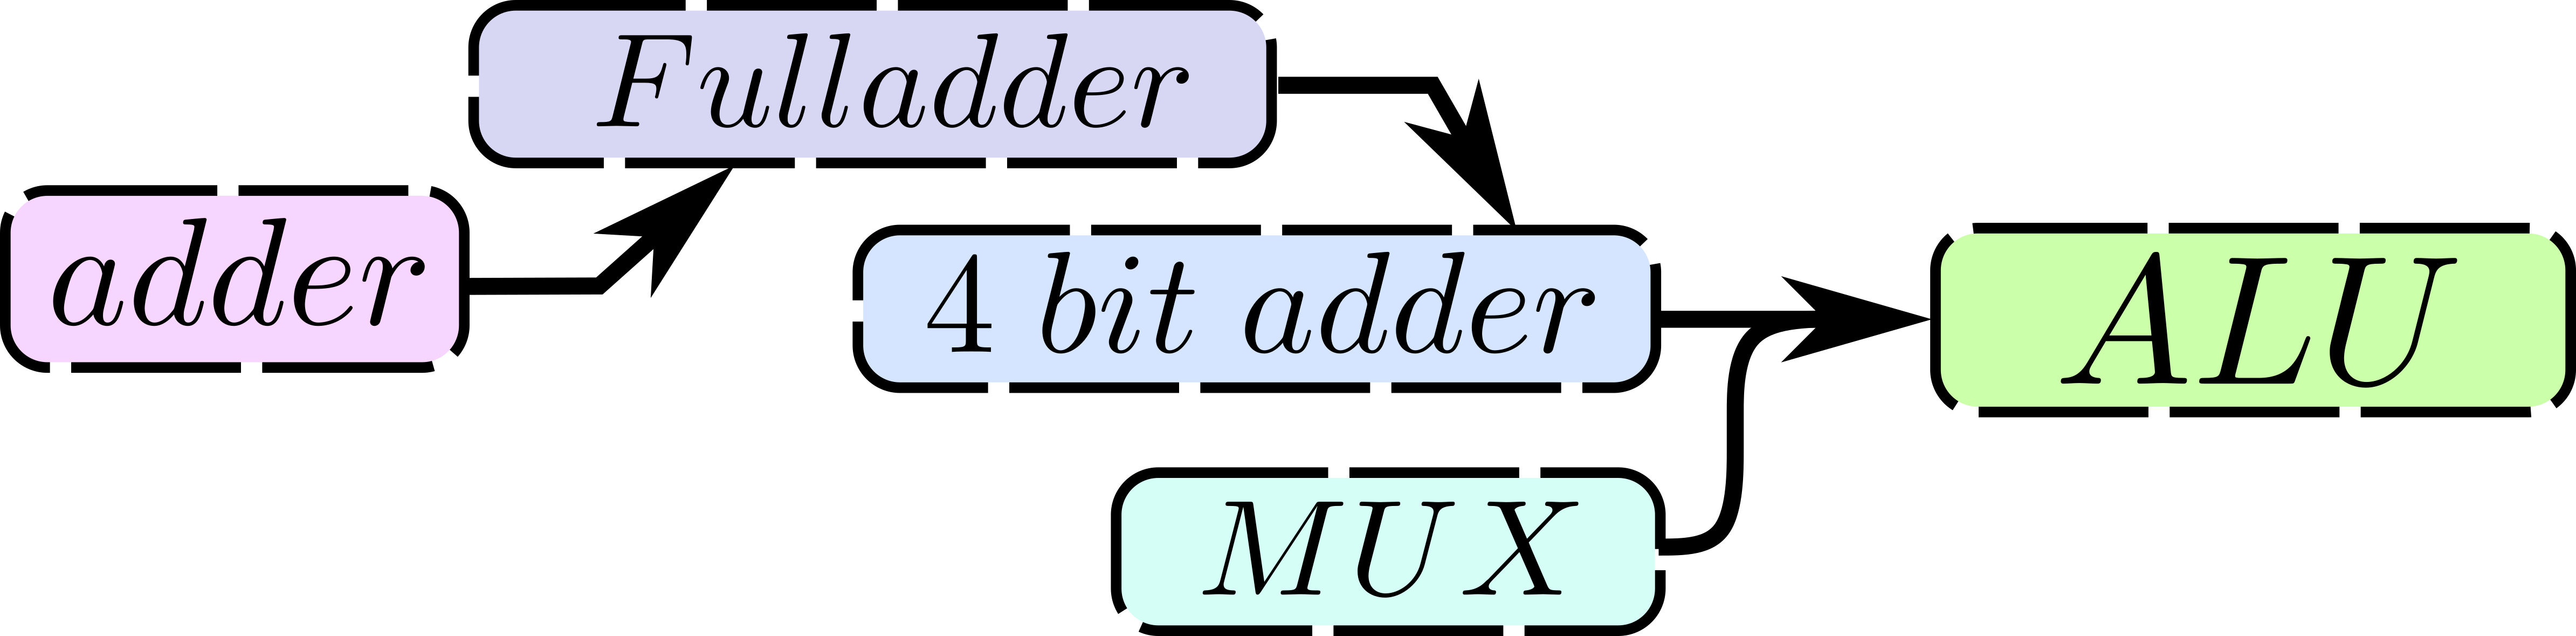
\includegraphics[scale=1]{data/modulos.png}
  \par\end{centering}
  \caption{Module dependencies}
\end{figure}
Each module has its own executable file to run their tests. The modules are

\begin{itemize}
  \item $Mux$: It connects the corresponding operation wire with corresponding output. It is an 8 input mux with inputs of size 4.
  \item $4\;bit\;adder$: Its function is to add 4 bit numbers and compute carry and overflow flags of that operations
  \item $Fulladder$: Adds 1 bit numbers with carry in, and carry out functionality
  \item $Adder $: Basic one bit number adder with carry functionality
\end{itemize}

Currently sum and substract are built from scratch, other operations use verilog built-in fucntions, altough, it would not cause any compatibility problem to have these functions manually coded.

Now we will analize in more depth how the program works

\subsection*{ALU overview}

\begin{figure}[H]
  \begin{centering}
  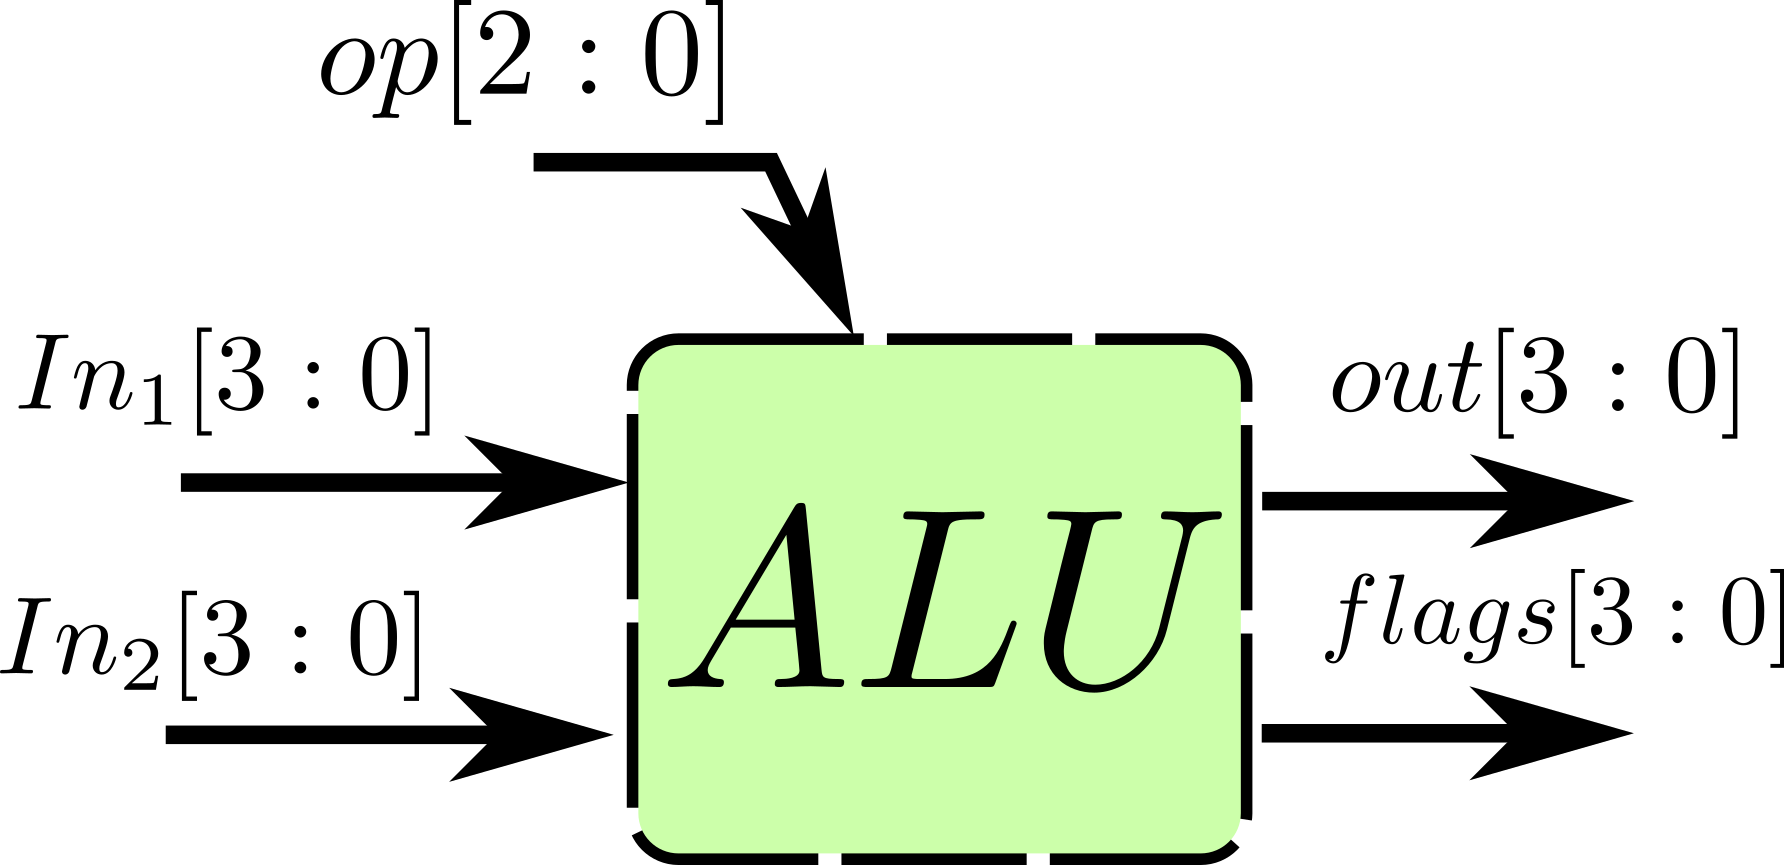
\includegraphics[scale=1]{data/alu.png}
  \par\end{centering}
  \caption{Alu in-out}
\end{figure}

The ALU makes sure the output and flags are correct accoring to opcodes and inputs.
\subsection*{Operations}
There are 8 operations
\begin{itemize}
  \item \textbf{addition} (000) : Implemented using 4 bit full adder
  \item \textbf{difference} (001): Implemented using 4 bit full adder using carry in and built-in not operator
  \item \textbf{and} (010): Implemented with built-in function
  \item \textbf{or} (011): Implemented with built-in function
  \item \textbf{not} (100): Implemented with built-in function
  \item \textbf{xor} (101): Implemented with built-in function
  \item \textbf{2'th complement} (110): Implemented with built-in function
  \item \textbf{shift left} (111): Implemented with built-in function
\end{itemize}

All 8 operations are connected into a wire array, then Mux comes into action and select according to opcode which action write to output
Also another important detail is that operations that use only one number use input 1, and ignore input 2

There are four flags
\begin{itemize}
  \item \textbf{carry/overflow} (Managed by 4 bit adder modules)
  \item \textbf{zero/negative} (Easily managed directly by ALU)
\end{itemize}
It is important to note that operations that do not use carry and overflow make these bits to be 0.

\subsection*{Mux}
\begin{figure}[H]
  \begin{centering}
  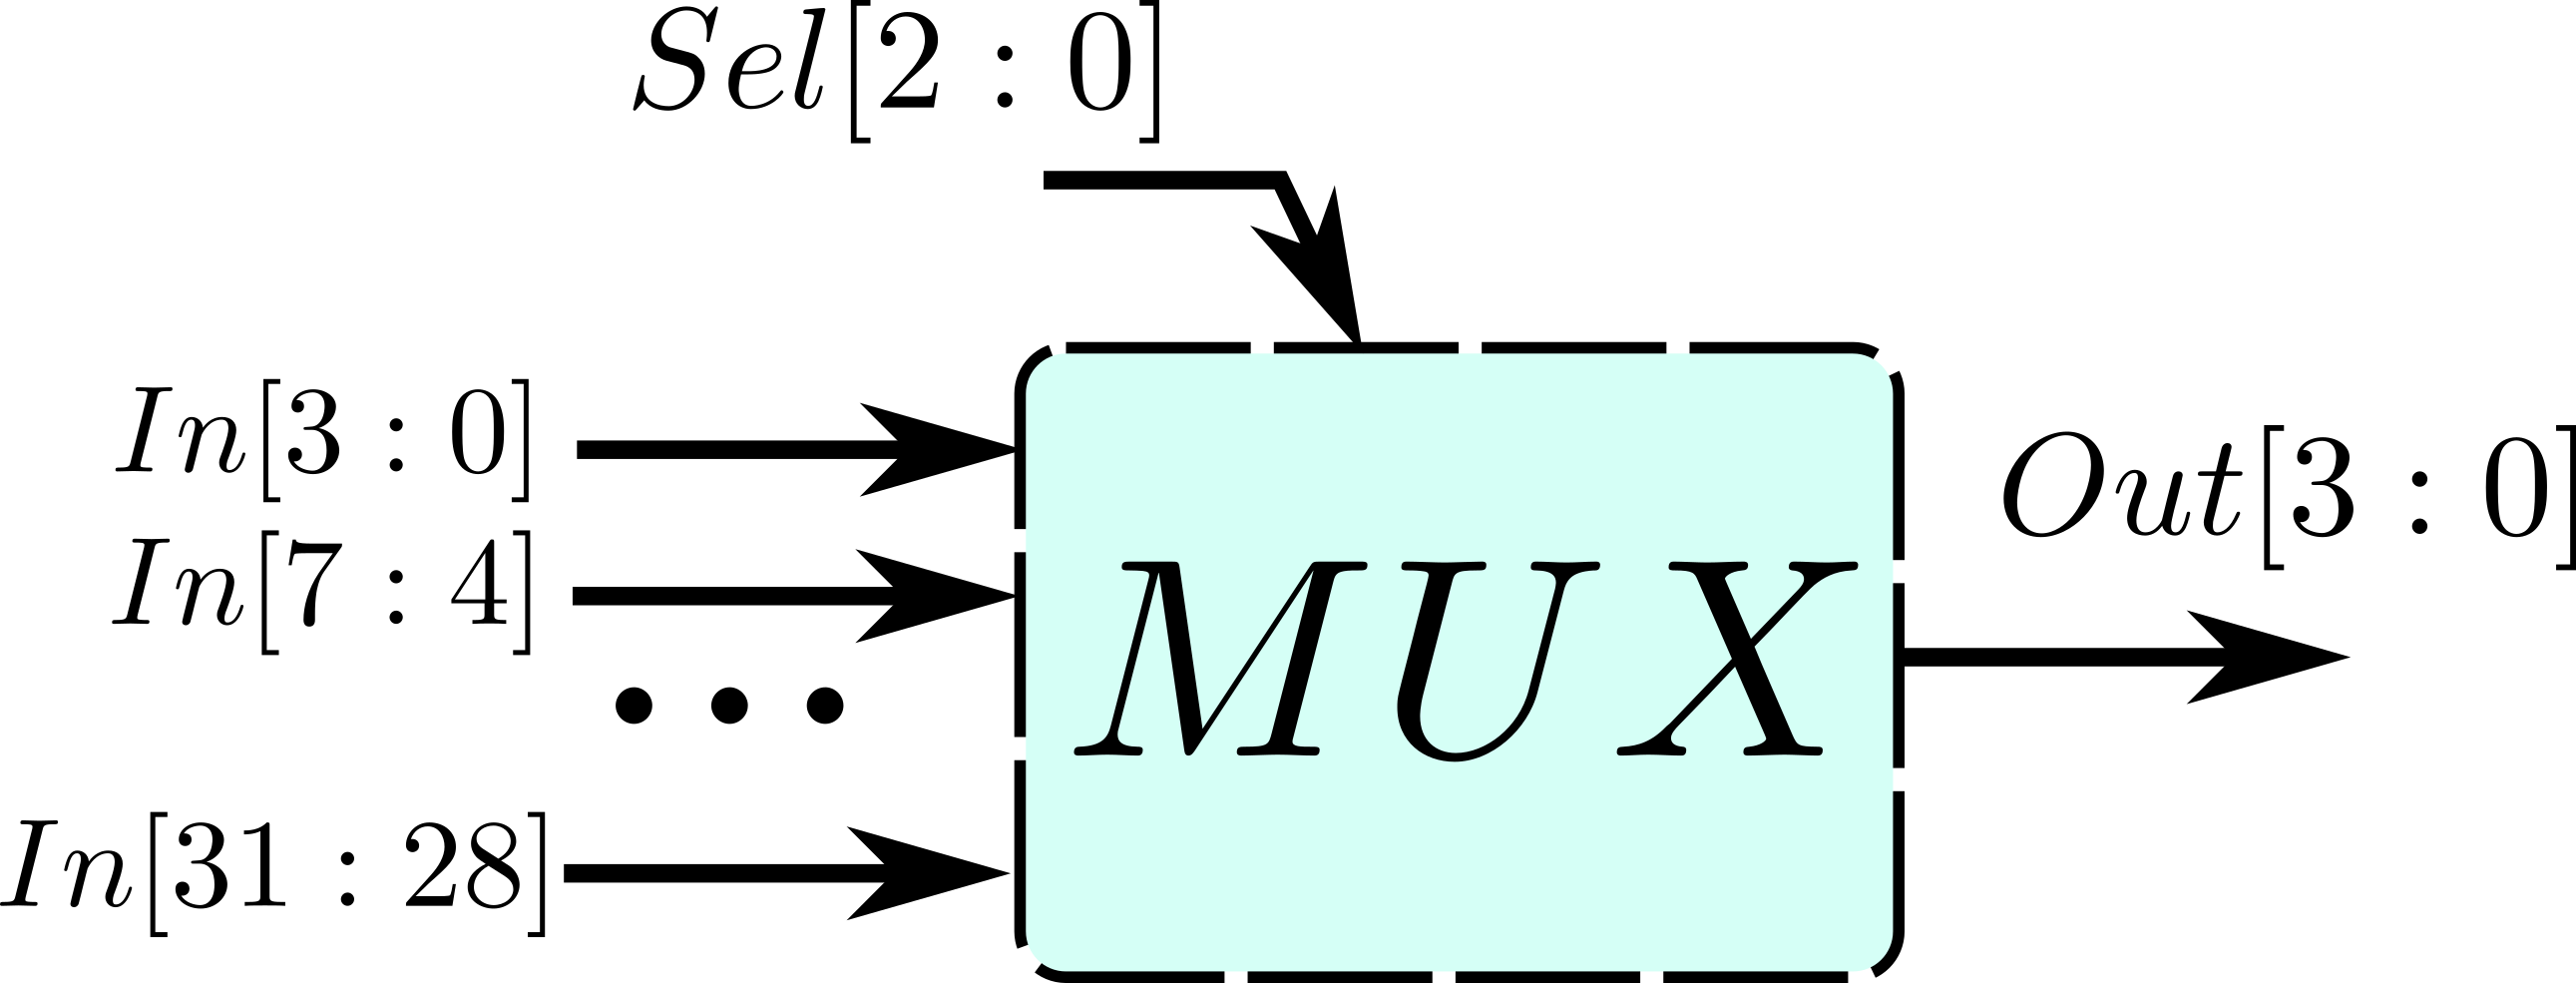
\includegraphics[scale=1]{data/mux.png}
  \par\end{centering}
  \caption{Mux in-out}
\end{figure}

This is a very simple module, implemented using vectorized expresions. It justs decides which input is wired to output according to selector input

\subsection*{Full 4bit Adder}

\begin{figure}[H]
  \begin{centering}
  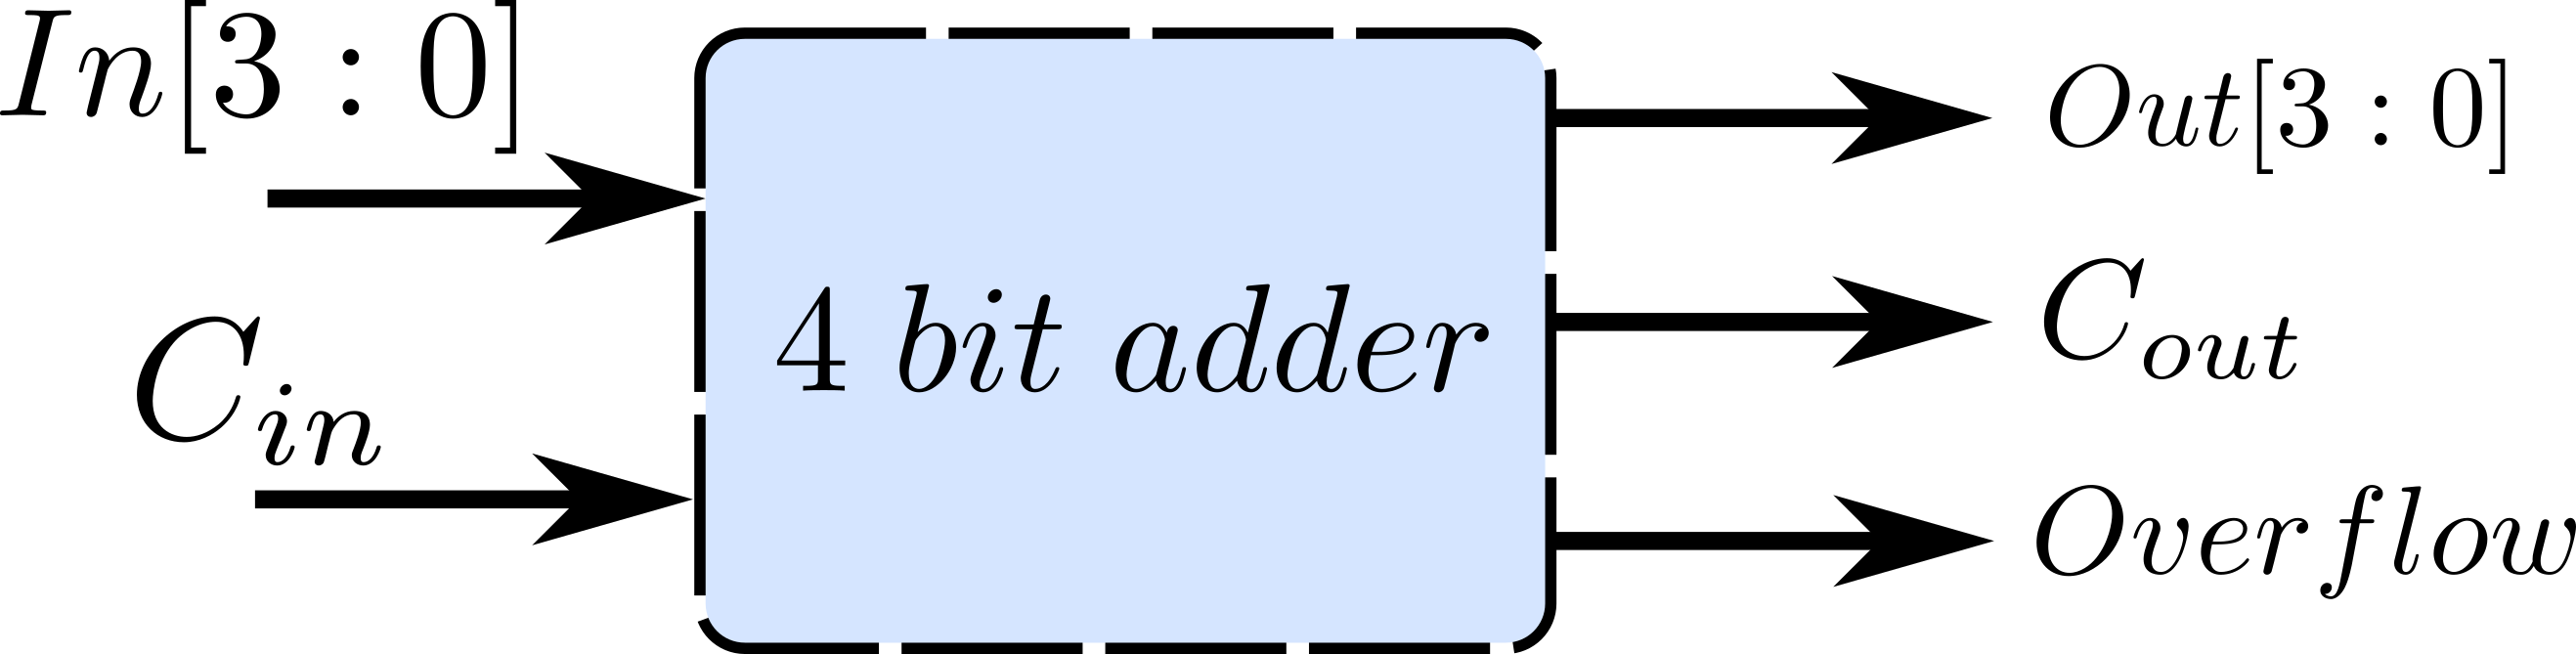
\includegraphics[scale=1]{data/4bitadder.png}
  \par\end{centering}
  \caption{Full 4bit Adder in-out}
\end{figure}

This module adds two binary 4 bit number with carry-in, carry-out functionality. Also it computes the overflow flag by making the xor of the 'last bit' carry and the carry-out
Also , to function this module uses 4 single full adders connected in 	
cascade. We won't describe these modules in this file because they are standard and the sources are enough.


